\section*{Ziel}
    In diesem Versuch sollen die Dichte, Rauigkeit und Schichtdicke eines Films auf einem Siliziumwafer mithilfe von Röntgenstrahlung bestimmt werden.
\section{Theorie}
    \label{sec:theorie}
    \subsection{Röntgenröhre}
        Um Röntgenstrahlung zu erzeugen kann eine sogenannte Röntgenröhre verwendet werden.
        Eine Röntgenröhre besteht im Wesentlichen aus einer Kathode die Elektronen emittiert und einer Anode auf der die beschleunigten Elektronen eintreffen und Strahlung erzeugen.
        Um die Elektronen von der Kathode zur Anode zu beschleunigen wird eine Hochspannung an die beiden Bauteile angeschlossen.
        Um Wechselwirkungen der Elektronen mit der Luft zu verhindern ist es außerdem notwendig die Anode und Kathode in ein gemeinsames Vakuum einzuschließen.
        Wenn die beschleunigten Elektronen auf die Anode treffen werden drei Arten von Strahlung erzeugt, die  charakteristische Röntgenstrahlung, die Bremsstrahlung und die Lilienfeldstrahlung.

        Charakteristische Röntgenstrahlung ist abhängig von der Elektronenkonfiguration der Anode und entsteht dadurch, dass die beschleunigten Elektronen die Elektronen in den Energieniveaus des Anodenmaterials stoßen und aus einer niedrigen Schale entfernen.
        Für den Stoß muss dabei mindestens die Energie aufgewendet werden die für das jeweilige Elektron nötig ist um auf das nächste unbesetzte Energieniveau angeregt zu werden.
        Wenn nun das Elektron aus seinem Platz in der niedrigen Schale gestoßen wurde rückt ein Elektron von einem höheren Energieniveau in seinen Platz und die Energiedifferenz der Zustände wird in Form von Röntgenstrahlung abgestrahlt.

        Die Bremsstrahlung wird von den beschleunigten Elektronen erzeugt wenn diese in das Coulombfeld der Kerne des Anodenmaterials gelangen, denn durch das elektrische Feld der Kerne werden die Elektronen abgelenkt und bewegte Ladungen strahlen elektromagnetische Strahlung ab, welche in diesem Fall kontinuierliche Röntgenstrahlung ist.

        Die Lilienfeldstrahlung ist eine spezielle Art von Übergangsstrahlung und entsteht beim Übergang der Elektronen vom Vakuum ins Anodenmaterial. Allerdings handelt es sich bei der Lilienfeldstrahlung um sichtbare elektromagnetische Strahlung und sie ist daher hier nicht von Interesse.

        Durch die charakteristische Strahlung und die Bremsstrahlung wird mit einer RöntgenRöhre ein kontinuierliches Röntgenspektrum mit einigen Peaks der charakteristischen Energiedifferenzen des Anodenmaterials erzeugt.
    \subsection{Göbelspiegel}
        Um divergente Röntgenstrahlung zu bündeln und zu monochromatisieren werden sogenannte Göbelspiegel verwendet.
        Göbelspiegel bestehen aus mehreren schichten Parabolischen Spiegeln und können das Röntgenlicht bündeln und Monochromatisieren.
    \subsection{Brechung und Reflexion von Röntgenstrahlung}
        Röntgenstrahlen werden wie andere elektromagnetsche Strahlen auf Reflektiert und Gebrochen.
        Allerdings tritt bei Röntgenstrahlung die Besonderheit auf, dass der Realteil des Brechungsindex für Medien kleiner als Eins sein kann.
        Der Realteil kleiner Eins kommt zustande, da die Schwingungsfrequenz der Röntgenstrahlung höher ist als die der Elektronen im Medium.
        In diesem Fall kann die Phasengeschwindigkeit des Lichtes (aber nicht die Gruppengeschwindigkeit) einen Wert größer als die Lichtgeschwindigkeit $c$ annehmen.
        Um den Brechungsindex zu approximieren wird dabei folgende Formel verwendet:
        \begin{equation}
            n = 1-\delta+i\beta /; , \delta > 0
        \end{equation}
        Wobei $\delta$ einer kleinen (ca \num{e-6}) Korrektur entspricht und $\beta$ als Parameter die Absorption beschreibt.
        
        Wenn nun eine elektromagnetische Welle (in diesem Fall Röntgenstrahlung) aus dem Vakuum ($n = 0$) auf eine Grenzschicht zu einem Medium trifft wird ein Anteil der Welle mit einem Winkel $\alpha_r = \alpha_i$ reflektiert und der restliche Teil der Gesamtintensität transmittiert.
        Da für Röntgenstrahlung der Brechungsindex von Materie kleiner als Eins sein kann, wird das Medium für die Strahlung optisch dünner als das Vakuum und Totalreflexion ist möglich wenn die Strahlung mit einem kritisch kleinen Winkel einfällt.

        Um die das Reflexions- und Transmissionsverhalten der Wellle zu beschreiben werden die Fresnel\'schen Gleichungen genutzt.
        Im Allgemienen wird bei den Gleichungen zwischen einer polarisation senkrecht oder parallel zur einfallsebene unterschieden, bei Röntgenstrahlung muss dies aber nicht getan werden, da die Brechungsinizes nähreungsweise gleich sind.
        \begin{align}
            r = \frac{2n_1 \sin\left(\alpha_i\right)}{ n_1 \sin\left(\alpha_i\right) +n_2 \sin\left(\alpha_t\right) } \\
            t = \frac{2n_1 \sin\left(\alpha_i\right) - n_2 \sin\left(\alpha_t\right) }{ n_1 \sin\left(\alpha_i\right) +n_2 \sin\left(\alpha_t\right) }
        \end{align}
        Daher ergibt sich das Verhältnis der Intensitäten, die sogenannte Fresnel-Reflektivität zu 
        \begin{equation}
            R_F = |r|^2 = \frac{\left(\alpha_i - p_+\right)^2 + p_-^2}{\left(\alpha_i + p_+\right)^2 + p_-^2}
        \end{equation}
        mit
        \begin{equation}
            p_\pm^2 = \frac{1}{2} \left(\sqrt{\left( \alpha_i - \alpha_c\right)^2 + 4\beta^2} \pm \left( \alpha_i^2 - \alpha_c^2\right)\right)
        \end{equation}
        Für den Fall, dass $\alpha_i > 3\alpha_c$ so ist $R_F$ näherungsweise gegeben durch
        \begin{equation}
            R_F ≈ \left(\frac{\alpha_c}{2\alpha_i}\right)^4
        \end{equation}
    \subsection{Kiessig-Oszillationen}
        Im falle des Experiments haben wir kein ideales Medium unendlicher Tiefe, sondern ein Zweischichtensystem.
        Durch die Reflexion an beiden Grenzschichten können die emittierten Strahlen interferieren und das Muster kann Aufschluss über die Schichtdicke $d$ liefern.
        Dabei gilt
        \begin{align}
            2 d \sin\left(\alpha_i\right) = n\lambda\\
            d = \frac{2\pi}{\Delta q} ≈ \frac{\lambda}{2\Delta\alpha_i}
        \end{align}
        dabei steht q für den Wellenübertrag in z-Richtung und ergibt sich zu $q = 2k \sin\left(\alpha_i\right)$ mit dem Betrag des Wellenvektors $k$.
        Durch diese Interferenz oszilliert die Intensität der gemessenen ausfallenden Strahlung, wie in Abbildung \ref{fig:oszillation} zu sehen.
        \begin{figure}[ht]
            \centering
            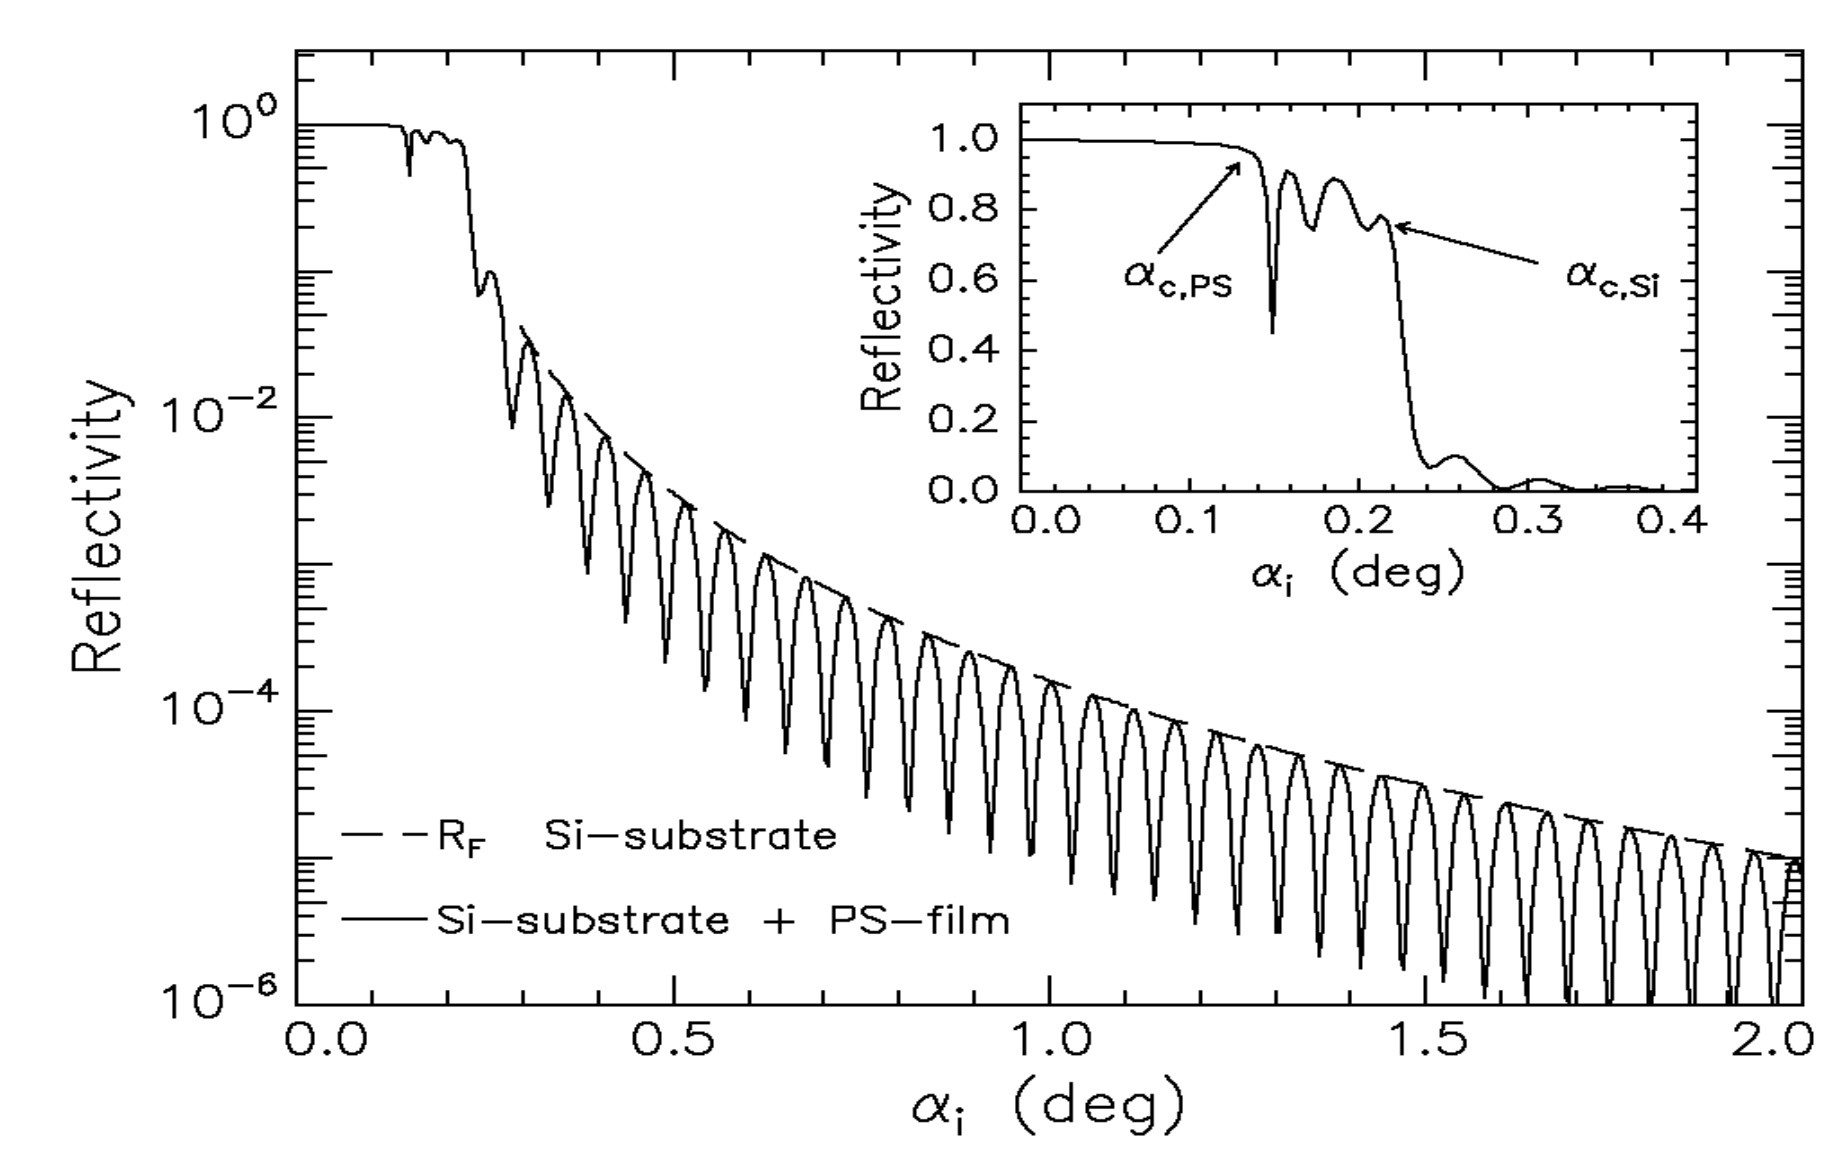
\includegraphics[width = 0.8\textwidth]{bilder/Oszillation.png}
            \caption{Oszillation}
            \label{fig:oszillation}
        \end{figure}
        Wenn die Ordnungszahl $m$ und der Winkel $\alpha_i$ für zwei Minima bekannt ist kann die Schichtdicke und die Dispersion und damit der Brechungsindex bestimmt werden.
        \begin{align}
            \delta = \frac{1}{2} \frac{\alpha_{i,1}^2 m_2^2 - \alpha_{i,2}^2 m_1^2}{m_2^2 -m_1^2}\\
            d = \frac{\lambda}{2\Delta\alpha_i}
        \end{align}
    \subsection{Parrat-Algorithmus}
        Im falle eines Mehrschichtensystems, siehe Abbildung \ref{fig:mehrschicht}, muss der sogenannte Parrat-Algorithmus verwendet werden um das System zu beschreiben.
        \begin{figure}[ht]
            \centering
            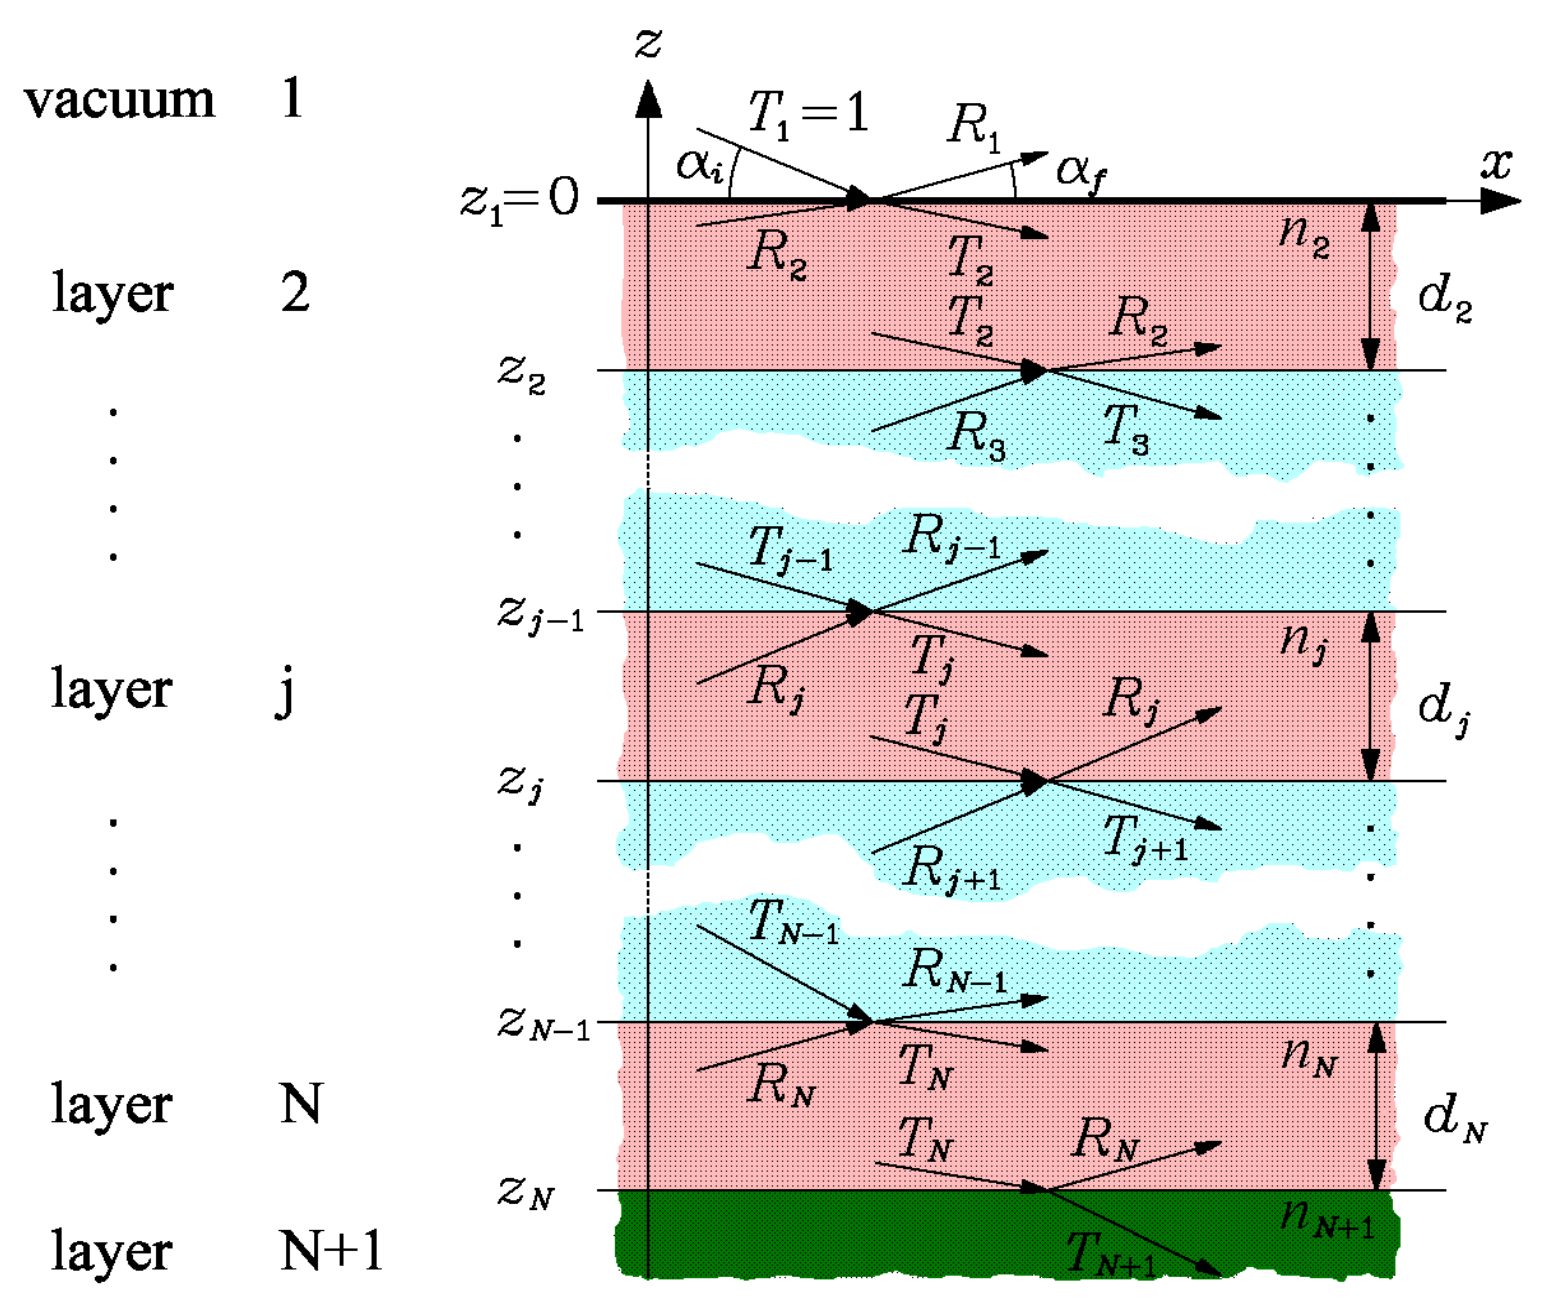
\includegraphics[width = 0.8\textwidth]{bilder/Mehrschichtsystem.png}
            \caption{Mehrschichtsystem}
            \label{fig:mehrschicht}
        \end{figure}
        Der Parrat-Algorithmus ist ein rekursiver Algorithmus zum berechnen des Verhaltnisses der reflektierten und transmittierten Welle an der j-ten Grenzschicht.
        \begin{align}
            X_j = \frac{j}{T_j} = e^{-2ik_{z,j}z_j} \frac{r_{j,j+1} + X_{j+1} e^{-2ik_{z,j+1}z_j}}{1 + r_{j,j+1}X_{j+1} e^{-2ik_{z,j+1}z_j}}\\
            r_{j,j+1} = \frac{k_{z,j} - k_{z,j+1}}{k_{z,j} + k_{z,j+1}}
        \end{align}
        wobei $r_{j,j+1}$ die Fresnelaktivität der j-ten Grenzfläche ist.
    \subsection{Rauigkeit}
        Im realen Fall sind Oberflächen nicht perfekt eben sondern haben eine Rauigkeit.
        Diese Rauigkeit kann theoretisch mit der root-mean-square-Rauigkeit beschrieben werden.
        \begin{equation}
            \sigma_j^2 = \int \left(z-z_j\right)^2\cdot P_j(z) \text{d}z        
        \end{equation}
        Dabei ist $P_j(z)$ die Wahrscheinlichkeit, dass die j-te Grenzfläche im Intervall $[z_j+z,z_j+z+\text{d}z]$ liegt.
        Beim Parrat Algorithmus werden dazu die Fresnelkoeffizienten modifiziert
        \begin{align}
            \tilde{r}_{j,j+1} = r_{j,j+1} e^{-2k_{z,j}k_{z,j+1} \sigma_j^2}\\
            \tilde{t}_{j,j+1} = t_{j,j+1} e^{ \frac{1}{2} \left(k_{z,j} -k_{z,j+1}\right)\sigma_j^2}
        \end{align}
